\documentclass
[
a4paper,                      % Format A4
twoside,					  % double sided, alternative: oneside
12pt,                         % font size
abstract,		      % include if you want to use the abstract environment (if there is an abstract)
fleqn,                        % equations are aligned on the left side, comment if you want centered equations
%BCOR=5mm,                     % indention on left side because of the binding
%cleardoubleplain              % page numbers are printed on empty pages, comment if this is not desired
]
{scrartcl} % KOMA script package for scientific articles
%-----------------------------------------------------------------------------------
% Packages (do not touch if you don't know what you are doing)
%-----------------------------------------------------------------------------------
% symbols and orthography
\usepackage[latin1]{inputenc} % symbol set 
\usepackage[english]{babel}   	% englisch orthography
%\usepackage[french]{babel}	   % french					
%\usepackage[ngerman]{babel}   % german
\usepackage[T1]{fontenc}      % enables "Umlaute" (not really needed for English)
\usepackage[scaled=.90]{helvet}
%----------------------
% Creative Commons License
\usepackage[scale=2]{ccicons}
%----------------------
% graphics
\usepackage{graphicx}         	% package to include graphics (pdf, png, jpg)
\usepackage{subfig}			% package for subfigures
\usepackage{float}            		% Option [H] for fixing floats where you want them to be (not recommended unless you really need it)
%------------------------------
% math packages
\usepackage[cmex10]{amsmath}  
\usepackage{amstext}          
\usepackage{amsfonts}        
\usepackage{amssymb}          
\usepackage{bm}               
%-----------------------------
\usepackage{hyperref}
%--------------------------------
% other packages
\usepackage{enumerate}        % better listings
\usepackage{booktabs}         % nicer tables (see manual for usage)
\usepackage{textcomp}         % for \textdegree , \textcelsius , sometimes causes problems
%\usepackage{algorithm}        % for including algorithms
%\usepackage{algorithmic}      % same as above, but other package (check the manual for usage) 
%\usepackage{theorem}          % for theorems
\usepackage{pdfpages}         % include whole pages from pdf files
\usepackage{parskip}          % insert an empty line between paragraphs instead of an indented beginning
\usepackage[right]{eurosym}   % Euro symbol
%\usepackage[hyphens]{url}     %enables line breaks for URLs \url{http://www}
% set border size of page (comment if you want Latex to do this)
\usepackage[inner=3cm,%
								outer=2cm,%
								top=2.7cm,%
								bottom=3.2cm]{geometry}
\usepackage{setspace}		  % for a different line spacing
\usepackage{multirow}
\usepackage{rotating}
\usepackage{xcolor,colortbl}

\definecolor{Gray}{gray}{0.85}
\definecolor{LightCyan}{rgb}{0.88,1,1}
%-----------------------------------------------------------------------------------
% other stuff (do not touch, it is good that way !)
%-----------------------------------------------------------------------------------
\sloppy                   % avoids lines that are too long on the right side
% avoid "orphans"
\clubpenalty = 10000
% avoid "widows"
\widowpenalty = 10000
% this makes the table of content etc. look better
\renewcommand{\dotfill}{\leaders\hbox to 5pt{\hss.\hss}\hfill}

% avoid indentation of line after a paragraph
\setlength{\parindent}{0pt}
%-----------------------------------------------------------------------------------
%-----------------------------------------------------------------------------------

%Header and footer settings
% 
\usepackage{scrpage2} % see manual for usage
\pagestyle{scrheadings}
\automark[section]{section}
\ofoot{\pagemark} % ofoo
\ifoot{Research Plan} % ofoo
%\cfoot[]{\pagemark}
%\ihead{}
%\ohead{}
%\ohead{\headmark}
%\setheadtopline{2pt}
%\setheadsepline{0.5pt}
%\setfootsepline{0.5pt}

%%%%%%%%%%%%%%%%%%%%%%%%%%%%%%%%%%%%%%%%%%%%%%%%%%%%%%%%%%%%%%%%%%%%%%%%%%%%%%%
%%%%%%%%%%%%%%%%%%%%%%%%%%%%%%%%%%%%%%%%%%%%%%%%%%%%%%%%%%%%%%%%%%%%%%%%%%%%%%
%
% References with BibTeX
%
\usepackage{natbib}
\bibliographystyle{apalike}
%\bibliographystyle{elsart-harv}
\setlength{\bibsep}{3mm}                  % spacing of the entries in the references
%
% look at the chapterbib package if you want to use a separate bibliography for each chapter
%
%%%%%%%%%%%%%%%%%%%%%%%%%%%%%%%%%%%%%%%%%%%%%%%%%%%%%%%%%%%%%%%%%%%%%%%%%%%%%%
%%%%%%%%%%%%%%%%%%%%%%%%%%%%%%%%%%%%%%%%%%%%%%%%%%%%%%%%%%%%%%%%%%%%%%%%%%%%%%
%
% some other stuff...
%
\setlength{\unitlength}{1cm}
\setlength{\oddsidemargin}{0.3cm}
\setlength{\evensidemargin}{0.3cm}
\setlength{\textwidth}{15.5cm}
\setlength{\topmargin}{0cm}
\setlength{\textheight}{22cm}
\columnsep 0.5cm

%%%%%%%%%%%%%%%%%%%%%%%%%%%%%%%%%%%%%%%%%%%%%%%%

% just compile particular parts
%
%\includeonly{./SUMMARY/summary} % put in here the path of the file you want to include only
%%%%%%%%%%%%%%%%%%%%%%%%%%%%%%%%%%%%%%%%%%%%%%%%%%%%%%%%%%%%%%%%%%%%%%%%%%%%%%

% define own commands
\newcommand{\brac}[1]{\left(#1\right)}		

%-----------------------------------------------------------------------------------%
%-----------------------------------------------------------------------------------%
%-----------------------------------------------------------------------------------%
%                                    START OF THE DOCUMENT                                %
%-----------------------------------------------------------------------------------%
%-----------------------------------------------------------------------------------%
%-----------------------------------------------------------------------------------%

\begin{document}

%------------------------------------------------%
%------------------------------------------------%
%                  Front Matter                         %
%------------------------------------------------%
%------------------------------------------------%

%------------------------------------------------%
%                 Title Page                               
%------------------------------------------------%

\clearscrheadings
\pagestyle{scrheadings}
\manualmark
%\ofoot{\pagemark} % ofoo
%\ifoot{Research Plan} % ofoo
%\cfoot[]{\pagemark}
%\ihead{}
%\ohead{}
\ihead{
\includegraphics[height=1.25cm]{logo-eeigm-ht90.png}\hspace{2.75cm}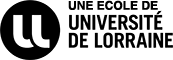
\includegraphics[height=1.25cm]{label-logo-ul.png}}
\ifoot{\noindent\makebox[\linewidth]{\rule{\textwidth}{0.4pt}}\\\textsc{EEIGM - 6, rue Bastien-Lepage BP 10630 - F-54010 Nancy Cedex}}

%\ohead{Abstract}
%\setheadtopline{2pt}
\setheadsepline{0.5pt}
%\setfootsepline{0.5pt}

\begin{center}

\vspace*{2cm}

\begin{Large}
\textbf{\textsc{EEIGM}}\\[0.75ex]
\end{Large}

\begin{large}
\textbf{\'Ecole Europ\'eenne d'Ing\'enieurs en G\'enie des Mat\'eriaux}\\[0.75ex]
\end{large}

\vspace{2cm}

\begin{large}
\textbf{$2^{`eme}$ Ann\'ee, $1^{er}$ Semestre}\\[0.75ex]
\end{large}
\vspace*{0.5cm}

\begin{Large}
\textbf{\textsc{M\'ecanique du Solide D\'eformable}}\\[0.75ex]
\end{Large}
\vspace*{0.5cm}

\begin{Large}
\textbf{\textsc{Notes de Cours}}\\[0.75ex]
\end{Large}
\vspace*{2.5cm}

\begin{large}
\textbf{Luca Di Stasio}\\[0.75ex]
\end{large}

\vspace{2cm}
%\begin{flushright}
%\begin{tabular}{l l }
%{\large \textbf{Author(s):}} & {\large Luca DI STASIO}\\
%\end{tabular}
%\end{flushright}

\begin{large}
\ccLogo\ccAttribution\ccNonCommercial\\[0.75ex]
Cette oeuvre est mise \`a disposition selon les termes de la\\ \href{https://creativecommons.org/licenses/by-nc/4.0/deed.fr}{Licence Creative Commons Attribution - Pas d'Utilisation Commerciale 4.0 International}.\\[0.75ex]
\end{large}

\vspace*{3cm}


{\large \textbf{6 ao\^ut 2020}}\\
%\textsc{DEFENSE LOCATION}\\

%------------------------------------------------
% Committee members:
%\textbf{\textsc{Committee Members}}\\[0.75ex]
%\textsc{NAME AND AFFILIATION}\\
%\textsc{NAME AND AFFILIATION}\\
%\textsc{NAME AND AFFILIATION}\\
%\textsc{ }\\

\end{center}

\newpage

%------------------------------------------------%
%            Table of Contents
%------------------------------------------------%

\pagenumbering{roman}

\setcounter{page}{1}

\clearscrheadings
\pagestyle{scrheadings}
\manualmark
\ofoot{\\ \pagemark} % ofoo
\ifoot{} % ofoo
%\cfoot[]{\pagemark}
%\ihead{}
%\ohead{}
\ohead{Contents}
\setheadtopline{2pt}
\setheadsepline{0.5pt}
\setfootsepline{0.5pt}

\tableofcontents 

\cleardoublepage

%------------------------------------------------%
%            List of Acronyms
%------------------------------------------------%

\clearscrheadings
\pagestyle{scrheadings}
\manualmark
\ofoot{\\ \pagemark} % ofoo
\ifoot{} % ofoo
%\cfoot[]{\pagemark}
%\ihead{}
%\ohead{}
\ohead{List of Acronyms}
\setheadtopline{2pt}
\setheadsepline{0.5pt}
\setfootsepline{0.5pt}

\section*{List of Acronyms}
\addcontentsline{toc}{section}{List of Acronyms}

\cleardoublepageusingstyle{scrheadings}

%------------------------------------------------%
%            List of Symbols
%------------------------------------------------%

\clearscrheadings
\pagestyle{scrheadings}
\manualmark
\ofoot{\\ \pagemark} % ofoo
\ifoot{} % ofoo
%\cfoot[]{\pagemark}
%\ihead{}
%\ohead{}
\ohead{List of Symbols}
\setheadtopline{2pt}
\setheadsepline{0.5pt}
\setfootsepline{0.5pt}

\section*{List of Symbols}
\addcontentsline{toc}{section}{List of Symbols}

\cleardoublepageusingstyle{scrheadings}

%------------------------------------------------%
%                       Abstract
%------------------------------------------------%

\clearscrheadings
\pagestyle{scrheadings}
\manualmark
\ofoot{\\ \pagemark} % ofoo
\ifoot{} % ofoo
%\cfoot[]{\pagemark}
%\ihead{}
%\ohead{}
\ohead{Abstract}
\setheadtopline{2pt}
\setheadsepline{0.5pt}
\setfootsepline{0.5pt}

\section*{Abstract}
\addcontentsline{toc}{section}{Abstract}

\cleardoublepageusingstyle{scrheadings}

%------------------------------------------------%
%------------------------------------------------%
%                   Main Matter                          %
%------------------------------------------------%
%------------------------------------------------%

\pagenumbering{arabic}

\setcounter{page}{1}

%------------------------------------------------%
%                   Introduction
%------------------------------------------------%

\clearscrheadings
\pagestyle{scrheadings}
\manualmark
\ofoot{\\\pagemark} % ofoo
\ifoot{} % ofoo
%\cfoot[]{\pagemark}
%\ihead{}
%\ohead{}
\ohead{Introduction}
\setheadtopline{2pt}
\setheadsepline{0.5pt}
\setfootsepline{0.5pt}

\section{Syst\`emes de coordonn\'ees curvilignes}

\subsection{\'Enonc\'e}

\subsection{Corrig\'e}

\cleardoublepageusingstyle{scrheadings}

\clearscrheadings
\pagestyle{scrheadings}
\manualmark
\ofoot{\\\pagemark} % ofoo
\ifoot{} % ofoo
%\cfoot[]{\pagemark}
%\ihead{}
%\ohead{}
\ohead{Second section}
\setheadtopline{2pt}
\setheadsepline{0.5pt}
\setfootsepline{0.5pt}

\section{Second section}

\cleardoublepageusingstyle{scrheadings}

%------------------------------------------------%
%------------------------------------------------%
%                   Back Matter                          %
%------------------------------------------------%
%------------------------------------------------%

\begin{appendix}

\clearscrheadings
\pagestyle{scrheadings}
\manualmark
\ofoot{\\\pagemark} % ofoo
\ifoot{} % ofoo
%\cfoot[]{\pagemark}
%\ihead{}
%\ohead{}
\ohead{Appendix A}
\setheadtopline{2pt}
\setheadsepline{0.5pt}
\setfootsepline{0.5pt}

\section{First appendix}

\cleardoublepageusingstyle{scrheadings}
%\cleardoublepage
\end{appendix}


% References
\clearscrheadings
\pagestyle{scrheadings}
\manualmark
\ofoot{\\\pagemark} % ofoo
\ifoot{} % ofoo
%\cfoot[]{\pagemark}
%\ihead{}
%\ohead{}
\ohead{References}
\setheadtopline{2pt}
\setheadsepline{0.5pt}
\setfootsepline{0.5pt}

\addcontentsline{toc}{section}{References}
\bibliography{}




\end{document}